\chapter{System Architecture Design}

Project details and descriptions also architectural design of project are explained in this chapter.

Mobile application will saved location, notes and media files also location of media files to storage when user start trip tracking feature of mobile application. Before starting a trip user can choose some of his/her friends to organize a trip with them when connected to Internet. If a person added a trip, this person will send an invitation notification which asks user to accept joining or reject joining to trip. If user accepted invitation he/she can join trip as a member. Inviter is accepted as leader of team. During the trip all user's behaviour saved separately. If location sharing feature opened any member of this team can watch other members location. However as we mentioned this feature requires Internet connection. At the end of trip when user want to share his/her trip data, path data will be provided from team leader but all of media data will be merged. All users can select the content that they want to share separately.

In order to save location on background, android application will use a location saving service. Using service is a must because, Android services can provide to execute a process for long time on the background. This application must to run location save service for long time. User can watch his/her location path on map during trip. If user wants to follow a path which is shared by another user, he/she can follow the path by looking at map.

\newpage

\section{Communication Design}

When user wants to share a trip, all of the trip contents will combined in a zip file. Combining all of the content in a zip file also provides to compress data. The trip zip file creating steps and zip file contents shown in Figure \ref{fig:creatingZipFile}.

\begin{figure}[!htbp]
\centering
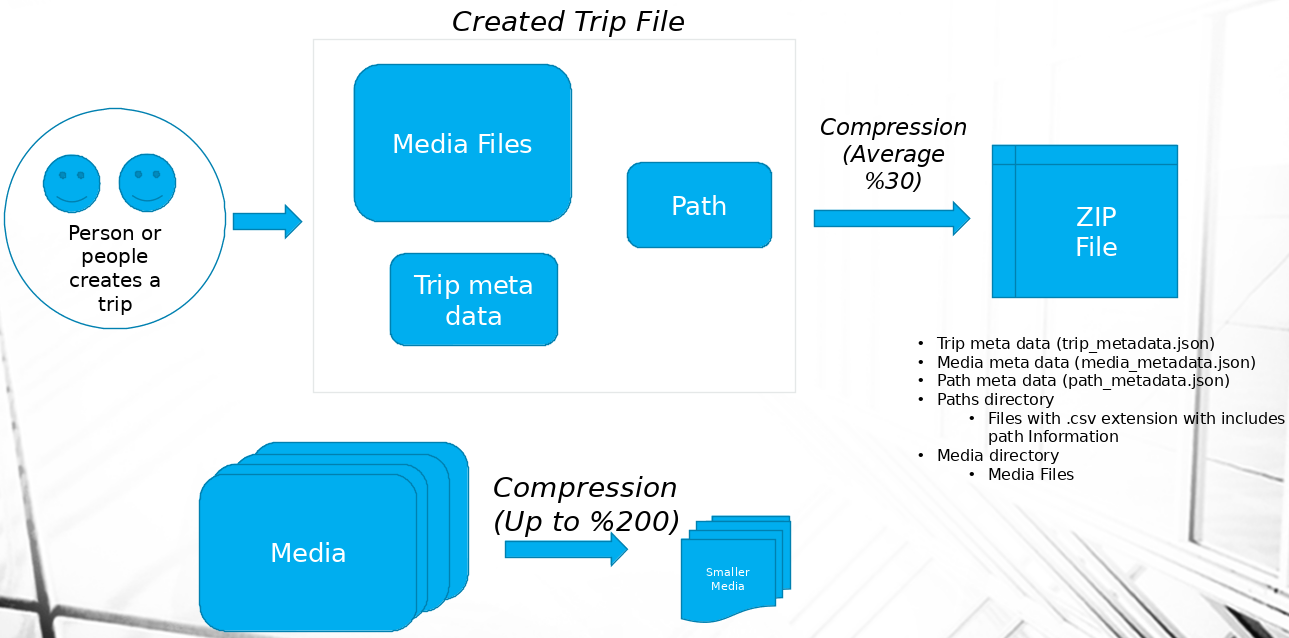
\includegraphics[width=\textwidth]{projectChapters/images/creatingZipFile.png}
\caption{Trip zip file creating steps and zip file contents}
\label{fig:creatingZipFile}
\end{figure}

An example of metadata files and path files in a zip file shown in Figure \ref{fig:metadata}.

\begin{figure}[!htbp]
\centering
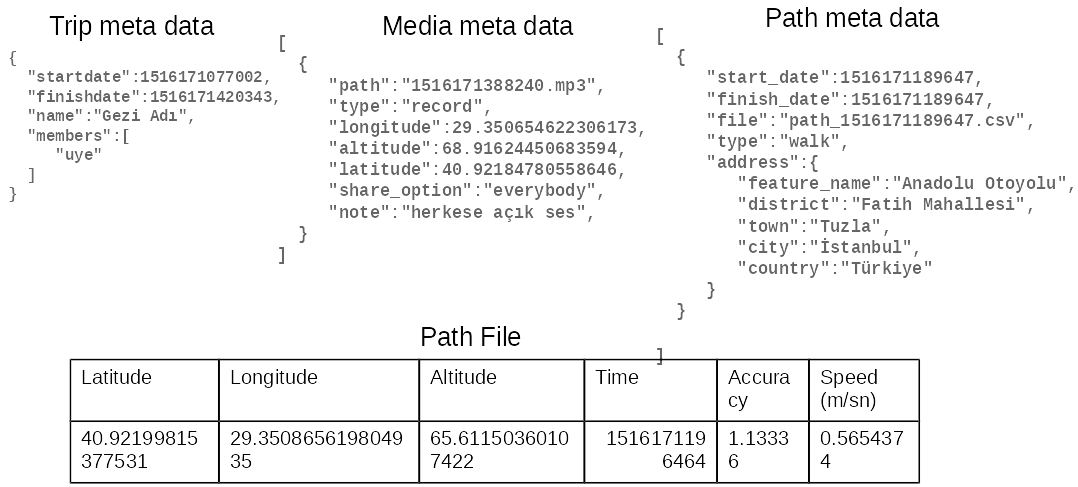
\includegraphics[width=\textwidth]{projectChapters/images/metadata.png}
\caption{Metadata files and Path files example}
\label{fig:metadata}
\end{figure}

\newpage

\section{Database Design}

Mobile Application database design shown in Figure \ref{fig:mobileApplicationDatabaseDiagram}.
\begin{figure}[!htbp]
\centering
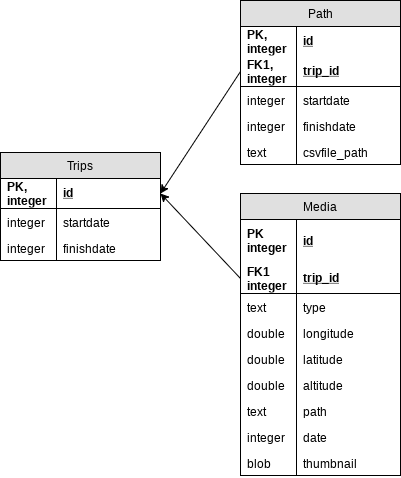
\includegraphics[width=\textwidth]{projectChapters/images/android_database.png}
\caption{Mobile Application Database Diagram}
\label{fig:mobileApplicationDatabaseDiagram}
\end{figure}

\begin{figure}[!htbp]
\centering
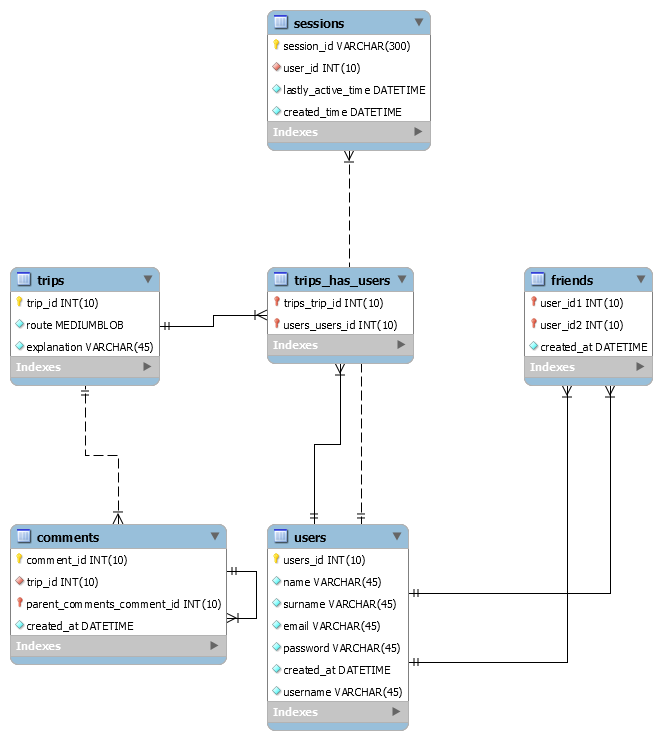
\includegraphics[width=40em, height=58em]{projectChapters/images/databaseDesign.png}
\caption{Server Side Database Diagram}
\label{fig:serverDatabase}
\end{figure}

Database designs of two different development side can be different in some aspects, the main reason of that server side also includes a social media platform which has more detailed information about users and the shared content. 

\newpage

\section{Modules}

There are system modules description in this section.

\subsection{User Register Module}
User register module provides creating new accounts, sends activation e-mails and activates user accounts. This module needs user name, password and e-mail from user to create a new account. This module runs on web application but user can use this module on mobile and web application.
\subsection{User Login Module}
User login module provides user to sing in into mobile and web application. This module needs user name and password from user to sing in. This module runs on web application but user can use this module on mobile and web application.
\subsection{User Password Reset Module}
This module provides password reset if the user forgets the password. This module available on both mobile and web application but this module runs on web application.
\subsection{Search Module}
This module provides user to search other users and shared trips by region, user, time and trip type. User can only search on trips which he/she have access rights to see. This module runs on web application but user can use this module on mobile and web application. 
\subsection{Location Save Module}
This module runs as a background task on Android device and saves navigation(longitude, latitude, altitude) data provided from GPS to a CSV file. This module runs on mobile application.
\subsection{Media Save Module}
This module saves photo, video and sound record with their location data to SQLite database on Android device. This module runs on mobile application.
\subsection{Feature Extraction Module}
This module tags trips using trip path data by their country, province, distinct, members, time and trip type on the web application. This module runs on mobile application.
\subsection{Trip Management Module}
This module provides user to manage trip contents like deleting a photo or changing access privileges for contents. This module runs on mobile application.
\subsection{Notification Sender Module}   
This module provides sending notifications to users about any topic. This module runs on web application but mobile application use this module as a web service.
\subsection{Trip Upload Module}
This module provides user to share trip content on social media with determined access rights. Mobile application prepares a zip file which includes all of contents belong to trip and upload this zip file to server side.
\subsection{Trip Download Module}
This module provides user to download chosen trip  which he/she can access to his/her mobile device using application. Web application prepares a zip file using chosen trip and chosen media files, after that sends it to mobile application.
\subsection{Team Trip Preparing Module}
This module provides users to send team trip requests each others. They can accept or deny these requests, if they accept they can contribute trips by sending their media. This module works on both mobile and web application.

\subsection{Team Content Merging Module}
This module provides trip members to merge trip content easily for share on social media. Web application merges all of sent contents from members in one trip. This module runs on web application.

\subsection{Team Members Location Tracking Module}
This module can only be used on team trips and requires Internet connection, provides team members to track each others locations simultaneously. This module runs on both mobile  and web application.
   
\subsection{Content Complaint Module}   
This module can be used both mobile device and web applications. Users can make complaint about other users, trips, comments. Created complaints are evaluated by the administrators. This module runs on server side but mobile application also interacts with it.
    
\subsection{Shared Content Interaction Module}    
This module can be used both on mobile application and web application. Users can like each others shared trip they can comment on those trips also can share the trips. This module runs on server side but mobile application also interacts with it.

\subsection{Administrator Module}
This module can only be used on web application. Administrator of system are able to interact with it, with the module administrators can evaluate created complaints by the users. Administrators can hide a content,user or comment if he or she thinks that complained content is inappropriate. This module runs on web side application.

\subsection{Users Interaction Module}
This module can be used both web and mobile application. Users can interact with other users by sending friend request, if they accept it they become friends and will be able see contents of each others. This module runs on web side application but can only be used both mobile and web applications.

\subsection{Media Supplementation Module}
This module provides user to add new media files to trip on stated location using Google map on web application. This module only runs on web application.


The dataflow diagrams are shown in Figure \ref{fig:roles}, \ref{fig:userdataflow}, \ref{fig:admindataflow}.


\begin{figure}[!htbp]
\centering
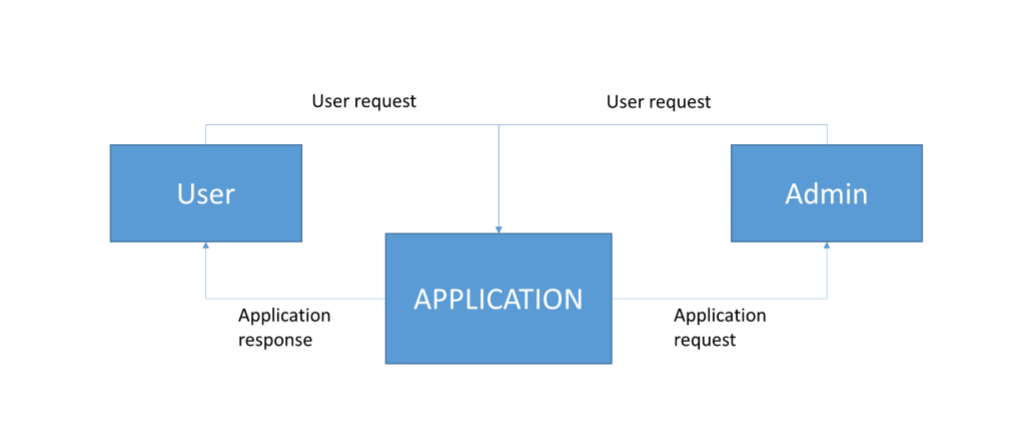
\includegraphics[width=\textwidth, height= 25em]{projectChapters/images/dataflow.png}
\caption{Level zero data flow diagram}
\label{fig:dataflow}
\end{figure}

\begin{figure}[!htbp]
\centering
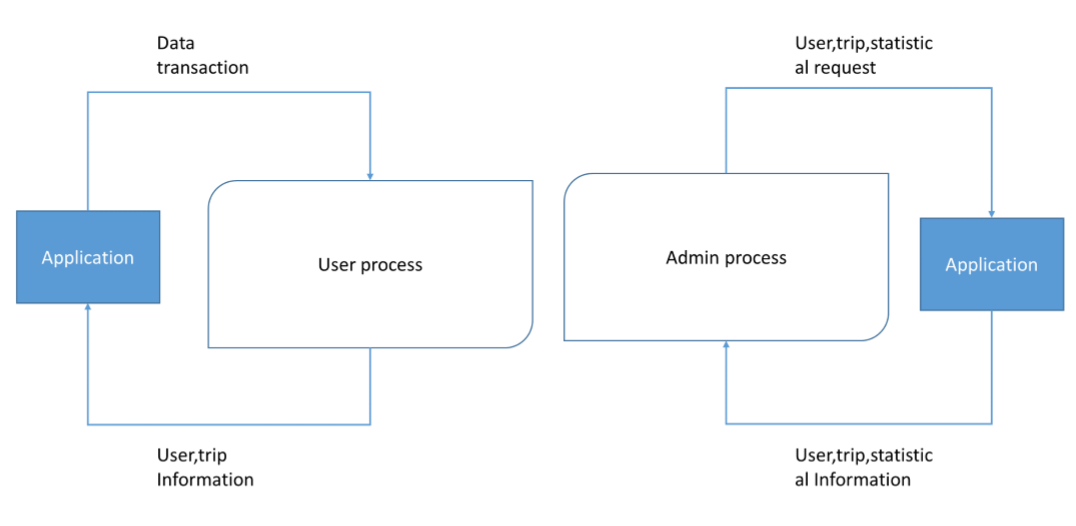
\includegraphics[width=\textwidth, height= 25em]{projectChapters/images/dataflow2.png}
\caption{Level one data flow diagram}
\label{fig:dataflow2}
\end{figure}

\begin{figure}[!htbp]
\centering
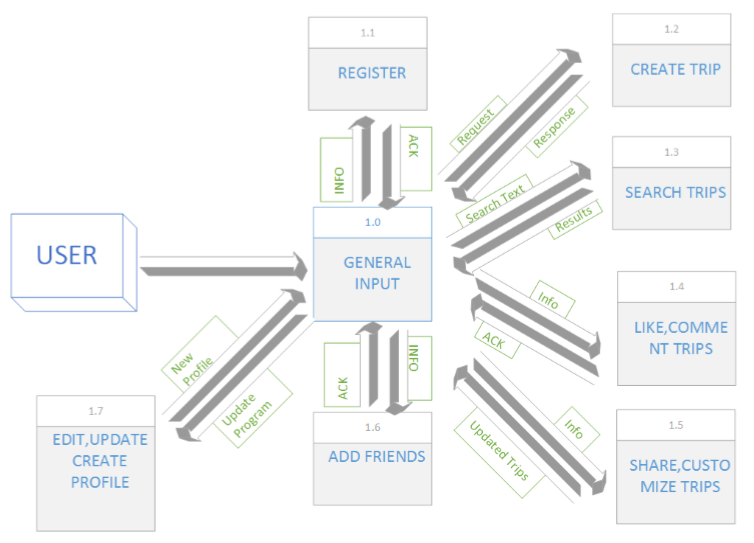
\includegraphics[width=\textwidth]{projectChapters/images/dataflow3.png}
\caption{Level two user data flow diagram}
\label{fig:userdataflow}
\end{figure}

\begin{figure}[!htbp]
\centering
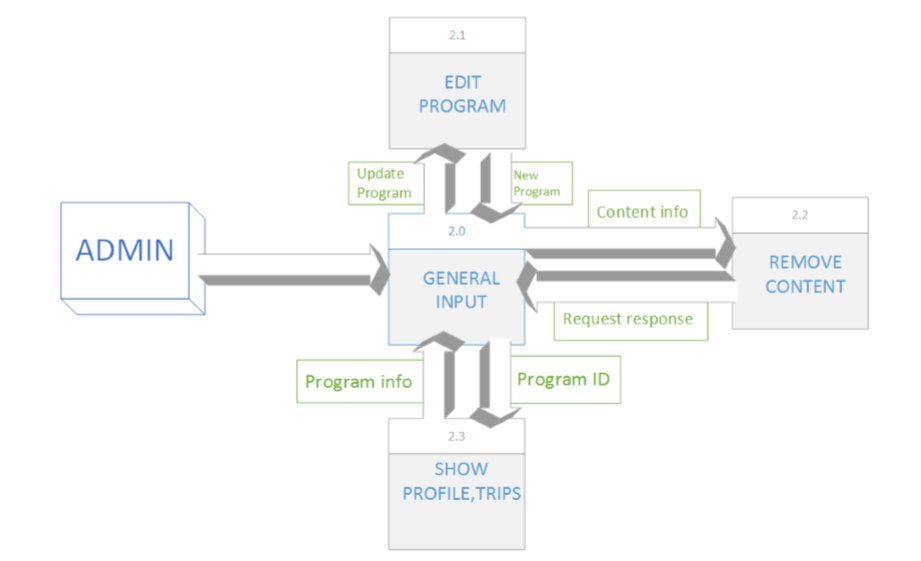
\includegraphics[width=\textwidth]{projectChapters/images/dataflow4.png}
\caption{Level two administrator data flow diagram}
\label{fig:admindataflow}
\end{figure}





